\documentclass[10pt]{article}
\usepackage[a4paper,margin=18mm]{geometry}
\usepackage{amsmath,amssymb,booktabs,array,enumitem,longtable}
\usepackage[T1]{fontenc}\usepackage{lmodern}
\usepackage{tikz}\usetikzlibrary{shapes.gates.logic.US,positioning,arrows.meta,patterns,calc}
\usepackage[hidelinks]{hyperref}
\setlength{\parindent}{0pt}\setlength{\parskip}{4pt}\setlength{\emergencystretch}{2em}
\newcommand{\VDD}{V_{DD}}
\newcommand{\mos}[4]{\begin{scope}[shift={(#1,#2)}]
\draw (0,.24)--(0,-.24);\draw (0,.20)--(.25,.20)--(.25,.5);
\draw (0,-.20)--(.25,-.20)--(.25,-.5);\draw (-.16,.23)--(-.16,-.23);
\ifnum#4=1\draw (-.26,0) circle (.06);\draw (-.75,0)--(-.32,0);\else\draw (-.75,0)--(-.16,0);\fi
\node[anchor=east,font=\scriptsize] at (-.76,0) {$#3$};\end{scope}}
\newcommand{\ground}[2]{\draw (#1,#2)--(#1,{#2-.12});\draw ({#1-.17},{#2-.12})--({#1+.17},{#2-.12});\draw ({#1-.11},{#2-.20})--({#1+.11},{#2-.20});}
\newcommand{\rail}[3]{\draw (#1,#2)--(#1,{#2+.14});\node[above,font=\scriptsize] at (#1,{#2+.14}) {$#3$};}
\newcommand{\hmos}[4]{\begin{scope}[shift={(#1,#2)}]
\draw(-.24,0)--(.24,0);\draw(-.2,0)--(-.2,-.25)--(-.5,-.25);\draw(.2,0)--(.2,-.25)--(.5,-.25);
\draw(-.23,.16)--(.23,.16);
\ifnum#4=1\draw(0,.26)circle(.06);\draw(0,.32)--(0,.75);\else\draw(0,.16)--(0,.75);\fi
\node[below,font=\scriptsize]at(0,-.32){#3};\end{scope}}
\newcommand{\qheading}[1]{\par\medskip\textbf{#1}\par}

\newcommand{\mosR}[4]{\begin{scope}[shift={(#1,#2)}]
\draw(0,.24)--(0,-.24);\draw(0,.20)--(-.25,.20)--(-.25,.5);
\draw(0,-.20)--(-.25,-.20)--(-.25,-.5);\draw(.16,.23)--(.16,-.23);
\ifnum#4=1\draw(.26,0)circle(.06);\draw(.32,0)--(.75,0);\else\draw(.16,0)--(.75,0);\fi
\node[anchor=west,font=\scriptsize]at(.76,0){$#3$};\end{scope}}
\newcommand{\tg}[4]{\draw({#1-.25},{#2-.22})rectangle({#1+.25},{#2+.22});
\draw(#1,{#2+.28})circle(.06);\draw(#1,{#2+.34})--(#1,{#2+.58})node[above,font=\scriptsize]{$#3$};
\draw(#1,{#2-.22})--(#1,{#2-.58})node[below,font=\scriptsize]{$#4$};}
\begin{document}
\begin{center}{\Large\bfseries EE3032 Introduction to VLSI Design---Final}\\Fall 2018\end{center}
\small Editable reconstruction of printed questions F-1--F-3. Handwritten study annotations are excluded. Printed point allocations total 115; all eight questions are retained. Figures preserve connectivity and qualitative waveforms, with normalized geometry.\normalsize
\qheading{1. (30 points) Answer the following questions.}
\begin{enumerate}[label=(\alph*),leftmargin=7mm]
\item Explain the latchup phenomenon and list two approaches to alleviate the occurrence probability of latchup. (6 points)
\item List two requirements for drawing the layout of a cell in the standard cell library. (4 points)
\item What is soft error? (2 points)
\item The soft error rate of a circuit is increased with the increasing of operation frequency and the scaling down of technology node? Explain the reasons in terms of three effects: logical masking effect, electrical masking effect, and latch window effect. (6 points)
\item List two limitations of the dynamic logic. (4 points)
\item What are the core-limited design and the pad-limited design? (4 points)
\item What is the physical design? What is the goal of the design rule? (4 points)
\end{enumerate}
\qheading{2. (10 points)} Fig. 1 shows a domino logic realizing the Boolean function $Y=ABC$. Complete the following questions.
\begin{center}\begin{tikzpicture}[x=1cm,y=.8cm,font=\small]
\node[and gate US,draw,logic gate inputs=nn,minimum width=1cm,minimum height=1cm](a)at(0,1.5){};
\node[and gate US,draw,logic gate inputs=nn,minimum width=1cm,minimum height=1cm](b)at(2.8,1.5){};
\draw(a.input 1)--++(-.6,0)node[left]{$A$};\draw(a.input 2)--++(-.6,0)node[left]{$B$};
\draw(a.output)--(1.7,1.5)|-(b.input 1);\draw(b.input 2)--++(-.6,0)node[left]{$C$};\draw(b.output)--++(.6,0)node[right]{$Y$};
\draw(0,2.5)--(0,2.0)node[above,pos=0]{$\phi$};\draw(2.8,2.5)--(2.8,2.0)node[above,pos=0]{$\phi$};
\node at(1.4,.4){(a)};
\begin{scope}[xshift=6cm]\node[left]at(0,1){$\phi$};\draw(0,1)--(.3,1)--(.6,1.6)--(1.6,1.6)--(1.9,1)--(2.9,1)--(3.2,1.6)--(4.2,1.6)--(4.5,1);\node at(2.2,.4){(b)};\end{scope}
\end{tikzpicture}\\\small Figure 1: (a) Domino logic circuit (b) Clock waveform.\end{center}
\begin{enumerate}[label=(\alph*),leftmargin=7mm]
\item Draw the transistor-level schematic diagram of the domino logic. (3 points)
\item Assume that the $t_r$ (rise time) and $t_f$ (fall time) of each 2-input AND gate are 1 ns and 2 ns, respectively. How long is the minimum clock period of $\phi$ if the duty cycle of $\phi$ is 50\%? (4 points)
\item Assume that each transistor has the following characteristics: $C_d=0.1$ fF; $C_g=1$ fF; $I_{Lp}=1$ nA (PMOS leakage current); $I_{Ln}=2$ nA (NMOS leakage current). Also, the supply voltage is 1.8 V and the threshold voltage of logic 1 is 1.3 V. Could the circuit be operated correctly at the minimum clock period? Why? (3 points)
\end{enumerate}
\newpage
\qheading{3. (10 points)} Figure 2 shows a Schmitt trigger circuit. If you apply an input signal as shown in the left figure to the Schmitt trigger circuit, the circuit outputs the signal as shown in the right figure. Assume that $\beta_n=2\beta_p$; the turn-on equivalent resistance of $N_1$ transistor is $R$; the simple RC delay model is used to estimate the delay and $t_r=t_f=2RC$. Complete the following questions.
\begin{center}\begin{tikzpicture}[x=.64cm,y=.70cm,font=\small]
\mos{1}{5}{}{1}\mos{1}{4}{}{1}\mos{1}{2.5}{}{0}\mos{1}{1.5}{}{0}
\rail{1.25}{5.5}{V_{DD}}\ground{1.25}{1}\draw(1.25,3)--(1.25,3.5);\draw(1.25,3.25)--(5,3.25)node[right]{$V_{out}$};\fill(1.25,3.25)circle(1.5pt);
\draw(-.25,1.5)--(-.25,5)--(.25,5);\foreach\y in {4,2.5,1.5}{\draw(-.25,\y)--(.25,\y);}\draw(-1.1,3.3)--(-.25,3.3)node[pos=0,left]{$V_{in}$};
\node[right]at(1.5,5){$P_1$};\node[right]at(1.5,4){$P_2$};\node[right]at(1.5,2.5){$N_2$};\node[right]at(1.5,1.5){$N_1$};
\hmos{3}{4.75}{$P_3$}{1}\draw(1.25,4.5)--(2.5,4.5);\draw(3.5,4.5)--(4,4.5);\ground{4}{4.5}
\hmos{3}{2.25}{$N_3$}{0}\draw(1.25,2)--(2.5,2);\draw(3.5,2)--(4,2);\rail{4}{2}{V_{DD}}
\draw(3,3)--(3,3.25);\fill(3,3.25)circle(1.5pt);\draw(3,5.5)--(4.5,5.5)--(4.5,3.25);\fill(4.5,3.25)circle(1.5pt);
\draw(4.7,3.25)--(4.7,2.9);\draw(4.45,2.9)--(4.95,2.9);\draw(4.45,2.78)--(4.95,2.78);\ground{4.7}{2.78}\node[right]at(4.95,2.83){$C$};
\begin{scope}[xshift=-6.5cm]
\draw[->](0,0)--(4.5,0)node[right]{$t$};\draw[->](0,0)--(0,4.8)node[above]{$V_{in}$};
\draw plot[smooth]coordinates{(0,4)(.45,4)(1,2.8)(1.25,3.1)(1.65,1.1)(1.88,.7)(2.2,.7)(2.45,1.2)(2.7,2.2)(2.95,1.7)(3.38,4)(4,4)};
\draw[dashed](0,2.8)--(3.7,2.8);\draw[dashed](0,1.2)--(3.2,1.2);\node[left]at(0,4){$V_{DD}$};\node[left]at(0,2.8){$V_T^+$};\node[left]at(0,1.2){$V_T^-$};\node[left]at(0,0){0 V};
\foreach\x/\l in {1/1,1.65/2,2.45/3,3.25/4}{\draw[dashed](\x,0)--(\x,1.2);\node[below]at(\x,0){$t_\l$};}
\end{scope}
\begin{scope}[xshift=6.5cm]
\draw[->](0,0)--(4.5,0)node[right]{$t$};\draw[->](0,0)--(0,4.8)node[above]{$V_{out}$};\node[left]at(0,4){$V_{DD}$};\node[left]at(0,0){0 V};
\draw(0,0)--(1.65,0)--(1.9,4)--(3.25,4)--(3.5,0)--(4,0);\draw[dashed](1.65,0)--(1.65,4.4);\draw[dashed](3.25,0)--(3.25,4.4);\node[above]at(1.75,4.3){$t_r$};\node[above]at(3.4,4.3){$t_f$};\node[below]at(1.65,0){$t_2$};\node[below]at(3.25,0){$t_4$};
\end{scope}
\end{tikzpicture}\\\small Figure 2: A CMOS Schmitt trigger circuit and its qualitative input/output waveforms.\end{center}
\begin{enumerate}[label=(\alph*),leftmargin=7mm]
\item Let $V_{tn}=|V_{tp}|=0.4$ V, $V_{DD}=2.0$ V, $V_T^+=1.4$ V, and $V_T^-=0.6$ V. If the size of $N_1=100$ nm$/40$ nm, determine the sizes of the transistors $N_2,N_3,P_1,P_2$, and $P_3$. (5 points)
\item Let $V_{tn}=|V_{tp}|=0.6$ V, $V_{DD}=1.8$ V, $V_T^+=1.2$ V, and $V_T^-=0.6$ V. If an inverter is designed by removing the transistors $N_3$ and $P_3$, is the short-circuit power of the inverter larger or smaller than that of the Schmitt trigger circuit? Explain your answer. (5 points)
\end{enumerate}
\qheading{4. (15 points)} Draw the transistor-level schematic diagram of the Boolean function $f=\overline{A(BC+D)}$ using each of the following logic design styles: (1) Dynamic logic (5 points) (2) Fully differential logic (5 points) (3) Differential split-level logic (5 points).
\qheading{5. (15 points)} Figure 3 shows an NP-domino logic circuit. Assume that $\beta_n=2\beta_p$. Complete the following questions.
\begin{enumerate}[label=(\alph*),leftmargin=7mm]
\item What is the Boolean function of the NP-domino logic circuit? (5 points)
\item If the sizes of $P_1$ and $N_5$ are 80 nm$/20$ nm and 20 nm$/20$ nm, respectively, determine the sizes of the other transistors such that $t_r=t_f$ at nodes $X$ and $Y$. (5 points)
\item If the gate capacitance of $N_5$ is $C$, the supply voltage is $V_{DD}$, and the operation frequency is $f$, express the dynamic power consumed by the clock in terms of $V_{DD}$, $f$, and $C$. (5 points)
\end{enumerate}
\begin{center}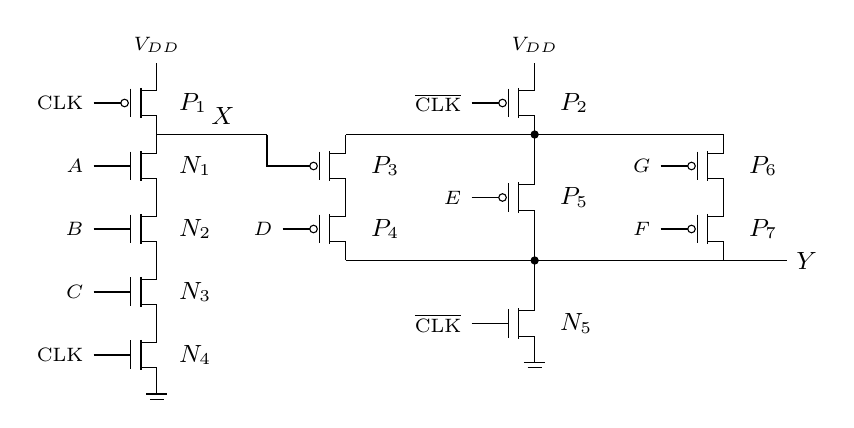
\begin{tikzpicture}[x=.8cm,y=.8cm,font=\small]
\mos{0}{6}{\mathrm{CLK}}{1}\rail{.25}{6.5}{V_{DD}}\mos{0}{5}{A}{0}\mos{0}{4}{B}{0}\mos{0}{3}{C}{0}\mos{0}{2}{\mathrm{CLK}}{0}\ground{.25}{1.5}
\draw(.25,5.5)--(2,5.5)node[above,pos=.6]{$X$};\node[right]at(.45,6){$P_1$};\node[right]at(.45,5){$N_1$};\node[right]at(.45,4){$N_2$};\node[right]at(.45,3){$N_3$};\node[right]at(.45,2){$N_4$};
\mos{6}{6}{\overline{\mathrm{CLK}}}{1}\rail{6.25}{6.5}{V_{DD}}
\draw(3.25,5.5)--(9.25,5.5);\fill(6.25,5.5)circle(1.5pt);\node[right]at(6.5,6){$P_2$};
\mos{3}{5}{}{1}\mos{3}{4}{D}{1}\mos{6}{4.5}{E}{1}\mos{9}{5}{G}{1}\mos{9}{4}{F}{1}
\draw(6.25,5)--(6.25,5.5);\draw(6.25,4)--(6.25,3.5);\draw(3.25,3.5)--(10.25,3.5)node[right]{$Y$};\fill(6.25,3.5)circle(1.5pt);
\draw(2,5.5)--(2,5)--(2.25,5);\node[right]at(3.5,5){$P_3$};\node[right]at(3.5,4){$P_4$};\node[right]at(6.5,4.5){$P_5$};\node[right]at(9.5,5){$P_6$};\node[right]at(9.5,4){$P_7$};
\mos{6}{2.5}{\overline{\mathrm{CLK}}}{0}\draw(6.25,3)--(6.25,3.5);\ground{6.25}{2}\node[right]at(6.5,2.5){$N_5$};
\end{tikzpicture}\\\small Figure 3: An NP-domino logic gate.\end{center}
\newpage
\qheading{6. (10 points)} Draw the transistor-level schematic diagram of the symbolic layout shown in Figure 4.
\begin{center}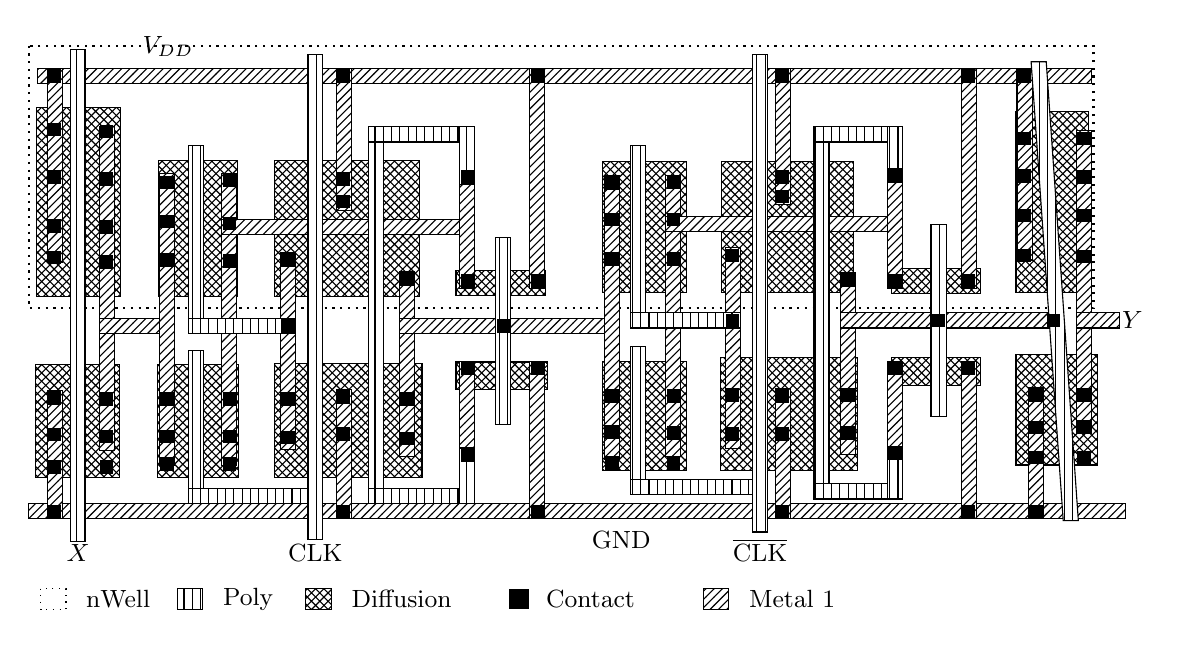
\begin{tikzpicture}[x=.012cm,y=-.012cm,font=\small]
\tikzset{lm/.style={preaction={fill=white},pattern=north east lines,pattern color=black},ld/.style={preaction={fill=white},pattern=crosshatch,pattern color=black},lp/.style={preaction={fill=white},pattern=vertical lines,pattern color=black}}
\draw[dotted,thick](273,108)rectangle(1400,386);
\draw[ld](281,173)rectangle(370,374);
\draw[ld](410,230)rectangle(494,374);
\draw[ld](533,230)rectangle(686,374);
\draw[ld](725,346)rectangle(820,373);
\draw[ld](880,231)rectangle(969,369);
\draw[ld](1006,231)rectangle(1146,369);
\draw[ld](1186,344)rectangle(1280,370);
\draw[ld](1318,178)rectangle(1395,369);
\draw[ld](280,446)rectangle(369,565);
\draw[ld](409,446)rectangle(495,565);
\draw[ld](533,445)rectangle(689,565);
\draw[ld](725,443)rectangle(822,472);
\draw[ld](880,442)rectangle(969,558);
\draw[ld](1005,438)rectangle(1150,558);
\draw[ld](1186,438)rectangle(1280,468);
\draw[ld](1318,435)rectangle(1404,552);
\draw[lm](282.0,132.0)rectangle(1398.0,148.0);
\draw[lm](272.0,593.0)rectangle(1434.0,609.0);
\draw[lm](292.0,132.0)rectangle(308.0,338.0);
\draw[lm](292.0,473.0)rectangle(308.0,609.0);
\draw[lm](347.0,194.0)rectangle(363.0,537.0);
\draw[lm](347.0,397.0)rectangle(427.0,413.0);
\draw[lm](411.0,243.0)rectangle(427.0,553.0);
\draw[lm](477.0,243.0)rectangle(493.0,553.0);
\draw[lm](477.0,292.0)rectangle(745.0,308.0);
\draw[lm](729.0,239.0)rectangle(745.0,365.0);
\draw[lm](539.0,327.0)rectangle(555.0,536.0);
\draw[lm](598.0,132.0)rectangle(614.0,283.0);
\draw[lm](598.0,472.0)rectangle(614.0,609.0);
\draw[lm](665.0,347.0)rectangle(681.0,543.0);
\draw[lm](665.0,397.0)rectangle(898.0,413.0);
\draw[lm](803.0,132.0)rectangle(819.0,365.0);
\draw[lm](803.0,442.0)rectangle(819.0,609.0);
\draw[lm](729.0,442.0)rectangle(745.0,550.0);
\draw[lm](882.0,246.0)rectangle(898.0,546.0);
\draw[lm](947.0,245.0)rectangle(963.0,543.0);
\draw[lm](947.0,289.0)rectangle(1198.0,305.0);
\draw[lm](1182.0,237.0)rectangle(1198.0,365.0);
\draw[lm](1010.0,322.0)rectangle(1026.0,535.0);
\draw[lm](1063.0,132.0)rectangle(1079.0,276.0);
\draw[lm](1063.0,471.0)rectangle(1079.0,609.0);
\draw[lm](1132.0,348.0)rectangle(1148.0,541.0);
\draw[lm](1132.0,391.0)rectangle(1366.0,407.0);
\draw[lm](1260.0,132.0)rectangle(1276.0,365.0);
\draw[lm](1260.0,442.0)rectangle(1276.0,609.0);
\draw[lm](1182.0,442.0)rectangle(1198.0,548.0);
\draw[lm](1319.0,132.0)rectangle(1335.0,335.0);
\draw[lm](1331.0,470.0)rectangle(1347.0,609.0);
\draw[lm](1382.0,198.0)rectangle(1398.0,519.0);
\draw[lm](1382.0,391.0)rectangle(1428.0,407.0);
\draw[lp](317.0,112.0)rectangle(333.0,633.0);
\draw[lp](442.0,214.0)rectangle(458.0,413.0);
\draw[lp](442.0,397.0)rectangle(555.0,413.0);
\draw[lp](442.0,431.0)rectangle(458.0,593.0);
\draw[lp](442.0,577.0)rectangle(584.0,593.0);
\draw[lp](568.0,117.0)rectangle(584.0,631.0);
\draw[lp](632.0,194.0)rectangle(648.0,593.0);
\draw[lp](632.0,194.0)rectangle(745.0,210.0);
\draw[lp](729.0,194.0)rectangle(745.0,255.0);
\draw[lp](632.0,577.0)rectangle(745.0,593.0);
\draw[lp](729.0,534.0)rectangle(745.0,593.0);
\draw[lp](767.0,311.0)rectangle(783.0,509.0);
\draw[lp](910.0,214.0)rectangle(926.0,407.0);
\draw[lp](910.0,391.0)rectangle(1026.0,407.0);
\draw[lp](910.0,427.0)rectangle(926.0,583.0);
\draw[lp](910.0,567.0)rectangle(1055.0,583.0);
\draw[lp](1039.0,117.0)rectangle(1055.0,623.0);
\draw[lp](1104.0,194.0)rectangle(1120.0,588.0);
\draw[lp](1104.0,194.0)rectangle(1198.0,210.0);
\draw[lp](1182.0,194.0)rectangle(1198.0,253.0);
\draw[lp](1104.0,572.0)rectangle(1198.0,588.0);
\draw[lp](1182.0,532.0)rectangle(1198.0,588.0);
\draw[lp](1228.0,297.0)rectangle(1244.0,501.0);
\draw[lp](1334,125)--(1350,125)--(1384,611)--(1368,611)--cycle;
\draw[fill=black](293.5,133.5)rectangle(306.5,146.5);
\draw[fill=black](293.5,594.5)rectangle(306.5,607.5);
\draw[fill=black](540.5,398.5)rectangle(553.5,411.5);
\draw[fill=black](730.5,240.5)rectangle(743.5,253.5);
\draw[fill=black](730.5,535.5)rectangle(743.5,548.5);
\draw[fill=black](768.5,398.5)rectangle(781.5,411.5);
\draw[fill=black](1011.5,392.5)rectangle(1024.5,405.5);
\draw[fill=black](1183.5,238.5)rectangle(1196.5,251.5);
\draw[fill=black](1183.5,533.5)rectangle(1196.5,546.5);
\draw[fill=black](1229.5,392.5)rectangle(1242.5,405.5);
\draw[fill=black](1351.5,392.5)rectangle(1364.5,405.5);
\draw[fill=black](599.5,133.5)rectangle(612.5,146.5);
\draw[fill=black](599.5,594.5)rectangle(612.5,607.5);
\draw[fill=black](804.5,133.5)rectangle(817.5,146.5);
\draw[fill=black](804.5,594.5)rectangle(817.5,607.5);
\draw[fill=black](1064.5,133.5)rectangle(1077.5,146.5);
\draw[fill=black](1064.5,594.5)rectangle(1077.5,607.5);
\draw[fill=black](1261.5,133.5)rectangle(1274.5,146.5);
\draw[fill=black](1261.5,594.5)rectangle(1274.5,607.5);
\draw[fill=black](1320.5,133.5)rectangle(1333.5,146.5);
\draw[fill=black](1332.5,594.5)rectangle(1345.5,607.5);
\draw[fill=black](293.5,190.5)rectangle(306.5,203.5);
\draw[fill=black](293.5,240.5)rectangle(306.5,253.5);
\draw[fill=black](293.5,292.5)rectangle(306.5,305.5);
\draw[fill=black](293.5,325.5)rectangle(306.5,338.5);
\draw[fill=black](348.5,192.5)rectangle(361.5,205.5);
\draw[fill=black](348.5,242.5)rectangle(361.5,255.5);
\draw[fill=black](348.5,293.5)rectangle(361.5,306.5);
\draw[fill=black](348.5,330.5)rectangle(361.5,343.5);
\draw[fill=black](412.5,246.5)rectangle(425.5,259.5);
\draw[fill=black](412.5,287.5)rectangle(425.5,300.5);
\draw[fill=black](412.5,328.5)rectangle(425.5,341.5);
\draw[fill=black](478.5,244.5)rectangle(491.5,257.5);
\draw[fill=black](478.5,289.5)rectangle(491.5,302.5);
\draw[fill=black](478.5,329.5)rectangle(491.5,342.5);
\draw[fill=black](540.5,328.5)rectangle(553.5,341.5);
\draw[fill=black](599.5,242.5)rectangle(612.5,255.5);
\draw[fill=black](599.5,266.5)rectangle(612.5,279.5);
\draw[fill=black](666.5,348.5)rectangle(679.5,361.5);
\draw[fill=black](730.5,350.5)rectangle(743.5,363.5);
\draw[fill=black](804.5,350.5)rectangle(817.5,363.5);
\draw[fill=black](883.5,247.5)rectangle(896.5,260.5);
\draw[fill=black](883.5,285.5)rectangle(896.5,298.5);
\draw[fill=black](883.5,327.5)rectangle(896.5,340.5);
\draw[fill=black](948.5,246.5)rectangle(961.5,259.5);
\draw[fill=black](948.5,285.5)rectangle(961.5,298.5);
\draw[fill=black](948.5,327.5)rectangle(961.5,340.5);
\draw[fill=black](1011.5,323.5)rectangle(1024.5,336.5);
\draw[fill=black](1064.5,240.5)rectangle(1077.5,253.5);
\draw[fill=black](1064.5,261.5)rectangle(1077.5,274.5);
\draw[fill=black](1133.5,349.5)rectangle(1146.5,362.5);
\draw[fill=black](1183.5,350.5)rectangle(1196.5,363.5);
\draw[fill=black](1261.5,350.5)rectangle(1274.5,363.5);
\draw[fill=black](1320.5,199.5)rectangle(1333.5,212.5);
\draw[fill=black](1320.5,239.5)rectangle(1333.5,252.5);
\draw[fill=black](1320.5,281.5)rectangle(1333.5,294.5);
\draw[fill=black](1320.5,323.5)rectangle(1333.5,336.5);
\draw[fill=black](1383.5,199.5)rectangle(1396.5,212.5);
\draw[fill=black](1383.5,240.5)rectangle(1396.5,253.5);
\draw[fill=black](1383.5,281.5)rectangle(1396.5,294.5);
\draw[fill=black](1383.5,324.5)rectangle(1396.5,337.5);
\draw[fill=black](293.5,474.5)rectangle(306.5,487.5);
\draw[fill=black](293.5,513.5)rectangle(306.5,526.5);
\draw[fill=black](293.5,547.5)rectangle(306.5,560.5);
\draw[fill=black](348.5,475.5)rectangle(361.5,488.5);
\draw[fill=black](348.5,515.5)rectangle(361.5,528.5);
\draw[fill=black](348.5,547.5)rectangle(361.5,560.5);
\draw[fill=black](412.5,475.5)rectangle(425.5,488.5);
\draw[fill=black](412.5,515.5)rectangle(425.5,528.5);
\draw[fill=black](412.5,544.5)rectangle(425.5,557.5);
\draw[fill=black](478.5,475.5)rectangle(491.5,488.5);
\draw[fill=black](478.5,515.5)rectangle(491.5,528.5);
\draw[fill=black](478.5,544.5)rectangle(491.5,557.5);
\draw[fill=black](540.5,475.5)rectangle(553.5,488.5);
\draw[fill=black](540.5,516.5)rectangle(553.5,529.5);
\draw[fill=black](599.5,473.5)rectangle(612.5,486.5);
\draw[fill=black](599.5,512.5)rectangle(612.5,525.5);
\draw[fill=black](666.5,475.5)rectangle(679.5,488.5);
\draw[fill=black](666.5,517.5)rectangle(679.5,530.5);
\draw[fill=black](730.5,443.5)rectangle(743.5,456.5);
\draw[fill=black](804.5,443.5)rectangle(817.5,456.5);
\draw[fill=black](883.5,472.5)rectangle(896.5,485.5);
\draw[fill=black](883.5,510.5)rectangle(896.5,523.5);
\draw[fill=black](883.5,543.5)rectangle(896.5,556.5);
\draw[fill=black](948.5,472.5)rectangle(961.5,485.5);
\draw[fill=black](948.5,511.5)rectangle(961.5,524.5);
\draw[fill=black](948.5,543.5)rectangle(961.5,556.5);
\draw[fill=black](1011.5,471.5)rectangle(1024.5,484.5);
\draw[fill=black](1011.5,512.5)rectangle(1024.5,525.5);
\draw[fill=black](1064.5,472.5)rectangle(1077.5,485.5);
\draw[fill=black](1064.5,512.5)rectangle(1077.5,525.5);
\draw[fill=black](1133.5,471.5)rectangle(1146.5,484.5);
\draw[fill=black](1133.5,511.5)rectangle(1146.5,524.5);
\draw[fill=black](1183.5,443.5)rectangle(1196.5,456.5);
\draw[fill=black](1261.5,443.5)rectangle(1274.5,456.5);
\draw[fill=black](1332.5,471.5)rectangle(1345.5,484.5);
\draw[fill=black](1332.5,505.5)rectangle(1345.5,518.5);
\draw[fill=black](1332.5,537.5)rectangle(1345.5,550.5);
\draw[fill=black](1383.5,471.5)rectangle(1396.5,484.5);
\draw[fill=black](1383.5,504.5)rectangle(1396.5,517.5);
\draw[fill=black](1383.5,537.5)rectangle(1396.5,550.5);
\node[above]at(420,130){$V_{DD}$};\node[below]at(900,612){GND};
\node[below]at(325,626){$X$};\node[below]at(576,626){CLK};\node[below]at(1047,620){$\overline{\mathrm{CLK}}$};\node[right]at(1420,399){$Y$};
\draw[dotted](285,683)rectangle(312,705);\node[right]at(323,694){nWell};
\draw[lp](430,683)rectangle(457,705);
\node[right]at(468,694){Poly};
\draw[ld](566,683)rectangle(593,705);
\node[right]at(604,694){Diffusion};
\draw[fill=black](782.0,684.0)rectangle(802.0,704.0);
\node[right]at(810,694){Contact};
\draw[lm](987,683)rectangle(1014,705);
\node[right]at(1025,694){Metal 1};
\end{tikzpicture}\\Figure 4: Symbolic layout.\end{center}
\small The vector redraw preserves the independently traced 2018 contacts, continuous poly routes and 20 active/poly crossings. Geometry is normalized; the source specifies no scale.\normalsize\par
\qheading{7. (10 points)} Figure 5 shows one possible implementation of the D register. Complete the following questions.
\begin{enumerate}[label=(\alph*),leftmargin=7mm]
\item Figure 5 shows a register consisting of a master latch and a low-cost slave latch. Label the clock signals for the transmission gates such that the register is a negative-edge triggered register. (3 points)
\item Assume that the delay of Inv1, Inv2, and the transmission gate is 0.15 ns, 0.2 ns, and 0.1 ns, respectively. Define the value of setup time of the register if the clock is ideal. (2 points)
\item As Figure 5 shows, assume that the switching threshold voltage of inverter Inv2 is $V_{DD}/2$ and the turn-on equivalent resistances of the transmission gate, N1, N2, P1, and P2 are $R_{TS},R_{N1},R_{N2},R_{P1}$, and $R_{P2}$, respectively. List two inequalities for determining the sizes of P2 and N2 such that the register can be operated correctly. (5 points)
\end{enumerate}
\begin{center}\begin{tikzpicture}[x=1cm,y=.95cm,font=\small]
\tg{1}{4.1}{}{}\tg{2.3}{1.4}{}{}\tg{6}{4.1}{}{}
\draw(0,4.1)--(.75,4.1)node[pos=0,left]{$D$};\draw(1.25,4.1)--(2,4.1);\draw(2,3.5)--(2,4.7)--(2.25,4.7);\draw(2,3.5)--(2.25,3.5);\fill(2,4.1)circle(1.5pt);
\mos{3}{4.7}{}{1}\mos{3}{3.5}{}{0}\rail{3.25}{5.2}{V_{DD}}\ground{3.25}{3}\draw(3.25,4.0)--(3.25,4.2);\draw(3.25,4.1)--(5.75,4.1);\fill(3.25,4.1)circle(1.5pt);
\node[right]at(3.5,4.7){$P_1$};\node[right]at(3.5,3.5){$N_1$};\draw[dotted](2.15,2.9)rectangle(3.95,5.5);\node[above]at(3,5.5){Inv1};
\mosR{4.5}{2}{}{1}\mosR{4.5}{.8}{}{0}\rail{4.25}{2.5}{V_{DD}}\ground{4.25}{.3}\draw(4.25,1.3)--(4.25,1.5);\draw(4.25,1.4)--(2.55,1.4);\draw(2.05,1.4)--(2,1.4)--(2,4.1);
\draw(4.6,4.1)--(5.5,4.1)--(5.5,.8)--(5.25,.8);\draw(5.5,2)--(5.25,2);\fill(4.6,4.1)circle(1.5pt);
\draw(6.25,4.1)--(6.6,4.1);\draw(6.6,4.1)--(7.15,4.1)--(7.15,4.7)--(7.25,4.7);\draw(7.15,4.1)--(7.15,3.5)--(7.25,3.5);\fill(6.6,4.1)circle(1.5pt);
\mos{8}{4.7}{}{1}\mos{8}{3.5}{}{0}\rail{8.25}{5.2}{V_{DD}}\ground{8.25}{3}\draw(8.25,4)--(8.25,4.2);\draw(8.25,4.1)--(9.5,4.1)node[right]{$Q$};
\draw[dotted](7.05,2.9)rectangle(8.7,5.5);\node[above]at(8,5.5){Inv2};
\mosR{8}{2}{}{1}\mosR{8}{.8}{}{0}\rail{7.75}{2.5}{V_{DD}}\ground{7.75}{.3}\draw(7.75,1.3)--(7.75,1.5);\draw(7.75,1.4)--(6.6,1.4)--(6.6,4.1);
\draw(9,4.1)--(9,.8)--(8.75,.8);\draw(9,2)--(8.75,2);\fill(9,4.1)circle(1.5pt);\node[left]at(7.5,2){$P_2$};\node[left]at(7.5,.8){$N_2$};
\end{tikzpicture}\\\small Figure 5: A static register. TG clock labels are intentionally blank, as in the original.\end{center}
\newpage
\qheading{8. (15 points)} Figure 6 shows a sequential circuit. Assume that the clock-to-Q propagation delay ($t_{pcq}$), the clock-to-Q contamination delay ($t_{ccq}$), the setup time ($t_{setup}$), and the hold time ($t_{hold}$) of the registers are 0.2 ns, 0.1 ns, 0.2 ns, and 0.2 ns, respectively. The delay of the XNOR gate, the AND gate, the OR gate, and the inverter is 0.4 ns, 0.5 ns, 0.5 ns, and 0.2 ns, respectively. Also, the delay of interconnection can be ignored. Complete the following questions.
\begin{enumerate}[label=(\alph*),leftmargin=7mm]
\item Can the circuit be operated correctly? If not, list two possible methods to modify the circuit such that it can operate correctly without sacrificing the operation frequency? Draw the modified circuit. (5 points)
\item Determine the maximum operation frequency of the modified circuit. (5 points)
\item Inserting registers into the circuit such that the modified circuit can be operated at $\frac43$ times the original operation frequency. (5 points)
\end{enumerate}
\begin{center}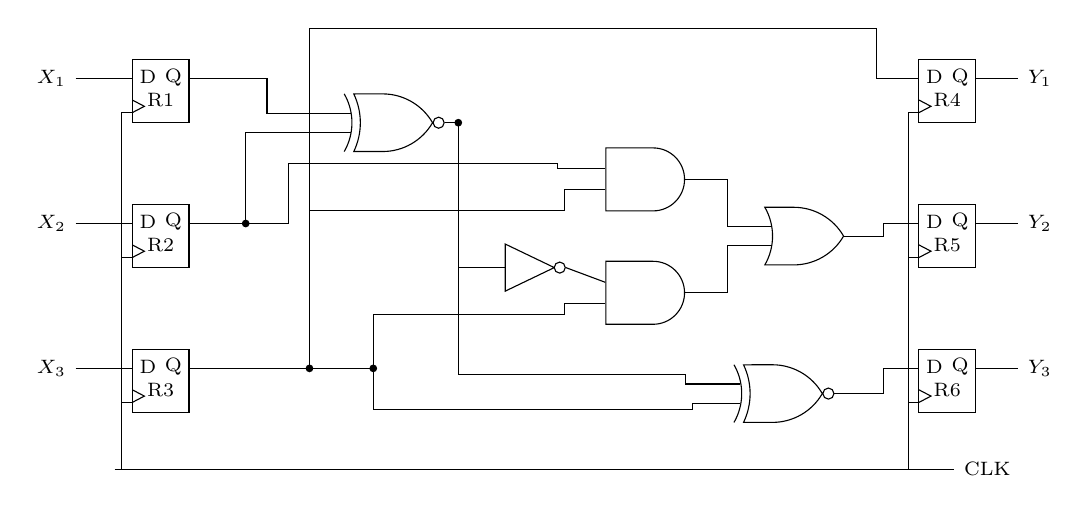
\begin{tikzpicture}[x=.9cm,y=.8cm,font=\scriptsize]
\draw(-0.4,5.5)rectangle(0.4,6.5);\node at(0,5.86){R1};\node at(-0.18,6.22){D};\node at(0.18,6.22){Q};\draw(-0.4,5.66)--(-0.23,5.76)--(-0.4,5.86);
\draw(10.7,5.5)rectangle(11.5,6.5);\node at(11.1,5.86){R4};\node at(10.92,6.22){D};\node at(11.28,6.22){Q};\draw(10.7,5.66)--(10.87,5.76)--(10.7,5.86);
\draw(-1.2,6.2)--(-.4,6.2)node[pos=0,left]{$X_1$};\draw(11.5,6.2)--(12.1,6.2)node[right]{$Y_1$};
\draw(-0.4,3.2)rectangle(0.4,4.2);\node at(0,3.56){R2};\node at(-0.18,3.9200000000000004){D};\node at(0.18,3.9200000000000004){Q};\draw(-0.4,3.3600000000000003)--(-0.23,3.46)--(-0.4,3.56);
\draw(10.7,3.2)rectangle(11.5,4.2);\node at(11.1,3.56){R5};\node at(10.92,3.9200000000000004){D};\node at(11.28,3.9200000000000004){Q};\draw(10.7,3.3600000000000003)--(10.87,3.46)--(10.7,3.56);
\draw(-1.2,3.9000000000000004)--(-.4,3.9000000000000004)node[pos=0,left]{$X_2$};\draw(11.5,3.9000000000000004)--(12.1,3.9000000000000004)node[right]{$Y_2$};
\draw(-0.4,0.8999999999999999)rectangle(0.4,1.9);\node at(0,1.2599999999999998){R3};\node at(-0.18,1.6199999999999999){D};\node at(0.18,1.6199999999999999){Q};\draw(-0.4,1.0599999999999998)--(-0.23,1.16)--(-0.4,1.2599999999999998);
\draw(10.7,0.8999999999999999)rectangle(11.5,1.9);\node at(11.1,1.2599999999999998){R6};\node at(10.92,1.6199999999999999){D};\node at(11.28,1.6199999999999999){Q};\draw(10.7,1.0599999999999998)--(10.87,1.16)--(10.7,1.2599999999999998);
\draw(-1.2,1.5999999999999999)--(-.4,1.5999999999999999)node[pos=0,left]{$X_3$};\draw(11.5,1.5999999999999999)--(12.1,1.5999999999999999)node[right]{$Y_3$};
\node[xnor gate US,draw,logic gate inputs=nn,minimum width=1cm](u)at(3.2,5.5){};
\draw(.4,6.2)--(1.5,6.2)|-(u.input 1);\draw(.4,3.9)--(1.2,3.9)|-(u.input 2);
\node[not gate US,draw,minimum width=.7cm](v)at(5.1,3.2){};
\draw(u.output)--(4.2,5.5)--(4.2,3.2)--(v.input);\fill(4.2,5.5)circle(1.4pt);
\node[and gate US,draw,logic gate inputs=nn,minimum width=1cm](p)at(6.8,4.6){};\node[and gate US,draw,logic gate inputs=nn,minimum width=1cm](r)at(6.8,2.8){};
\draw(1.2,3.9)--(1.8,3.9)--(1.8,4.85)--(5.6,4.85)|-(p.input 1);\fill(1.2,3.9)circle(1.4pt);
\draw(.4,1.6)--(2.1,1.6)--(2.1,4.1)--(5.7,4.1)|-(p.input 2);\fill(2.1,1.6)circle(1.4pt);
\draw(v.output)--(r.input 1);\draw(2.1,1.6)--(3,1.6)--(3,2.45)--(5.7,2.45)|-(r.input 2);\fill(3,1.6)circle(1.4pt);
\node[or gate US,draw,logic gate inputs=nn,minimum width=1cm](o)at(9,3.7){};\draw(p.output)--(8,4.6)|-(o.input 1);\draw(r.output)--(8,2.8)|-(o.input 2);\draw(o.output)--(10.2,3.7)|-(10.7,3.9);
\node[xnor gate US,draw,logic gate inputs=nn,minimum width=1cm](z)at(8.7,1.2){};\draw(4.2,5.5)--(4.2,1.5)--(7.4,1.5)|-(z.input 1);\draw(3,1.6)--(3,.95)--(7.5,.95)|-(z.input 2);\draw(z.output)--(10.2,1.2)|-(10.7,1.6);
\draw(2.1,4.1)--(2.1,7)--(10.1,7)|-(10.7,6.2);
\draw(-.65,0)--(11.2,0)node[right]{$\mathrm{CLK}$};\foreach\x in {-.55,10.55}{\foreach\y in {5.66,3.36,1.06}{\draw(\x,0)--(\x,\y)--++(.15,0);}}
\end{tikzpicture}\end{center}\begin{center}\small Figure 6: A sequential circuit. All six registers use a common ideal rising clock.\end{center}
\vfill\small Source footer: Li, EE, NCU; Fall 2018. This edition preserves the printed premises and point values.\end{document}
